\section{担当B — センサ処理・状態機械}

担当 B は，子機 Arduino における指揮者人形の観測・テンポ推定・状態管理を担う．
センサ構成はフォトトランジスタ（デジタル入力）とカラーセンサ（I2C）の 2 種類であり，
両センサの情報を組み合わせてテンポ推定と演奏開始判定を行い，発音タイミングを決定する．

\subsection{部品一覧}

\begin{table}[H]
\centering
\caption{使用部品一覧}
\label{tab:parts_B}
\begin{tabular}{p{4cm}p{5cm}p{2.5cm}p{3cm}}
\hline
\textbf{部品名} & \textbf{型番} & \textbf{ピン} & \textbf{用途} \\
\hline
フォトトランジスタ（$\times$5） & NJL7502L (560nm) & D4 & 拍タイミング検出（デジタル入力） \\
\hline
カラーセンサ（$\times$5） & AE\_S13683\_LED & I2C (SDA/SCL) & 演奏開始キュー（色）判別 \\
\hline
Arduino（子機） & Arduino Uno R4 WiFi & — & センサ処理・テンポ推定・状態管理 \\
\hline
\end{tabular}
\end{table}

\subsection{ハードウェア設計}

フォトトランジスタ（NJL7502L）はデジタルピン \texttt{D4} に接続し，
\texttt{HIGH} / \texttt{LOW} の二値で受光量を取得する．
カラーセンサ（AE\_S13683\_LED）はI2Cバス（SDA/SCL）に接続し，
ワンショット測定モードで RGB 値を取得する．

Arduinoと各デバイスのピン接続を表\ref{tab:pins_B}に示す．

\begin{table}[H]
\centering
\caption{ピン接続一覧}
\label{tab:pins_B}
\begin{tabular}{p{2.5cm}p{4cm}p{2.5cm}p{4cm}}
\hline
\textbf{Arduinoピン} & \textbf{接続先デバイス} & \textbf{信号種別} & \textbf{用途} \\
\hline
D4 (\texttt{PHOTO\_PIN}) & フォトトランジスタ & デジタル入力 & 拍タイミング検出 \\
\hline
SDA / SCL                & カラーセンサ（AE\_S13683\_LED） & I2C & 演奏開始キュー色判別 \\
\hline
\end{tabular}
\end{table}

図\ref{fig:circuit_B} に回路図を示す．

\begin{figure}[H]
\centering
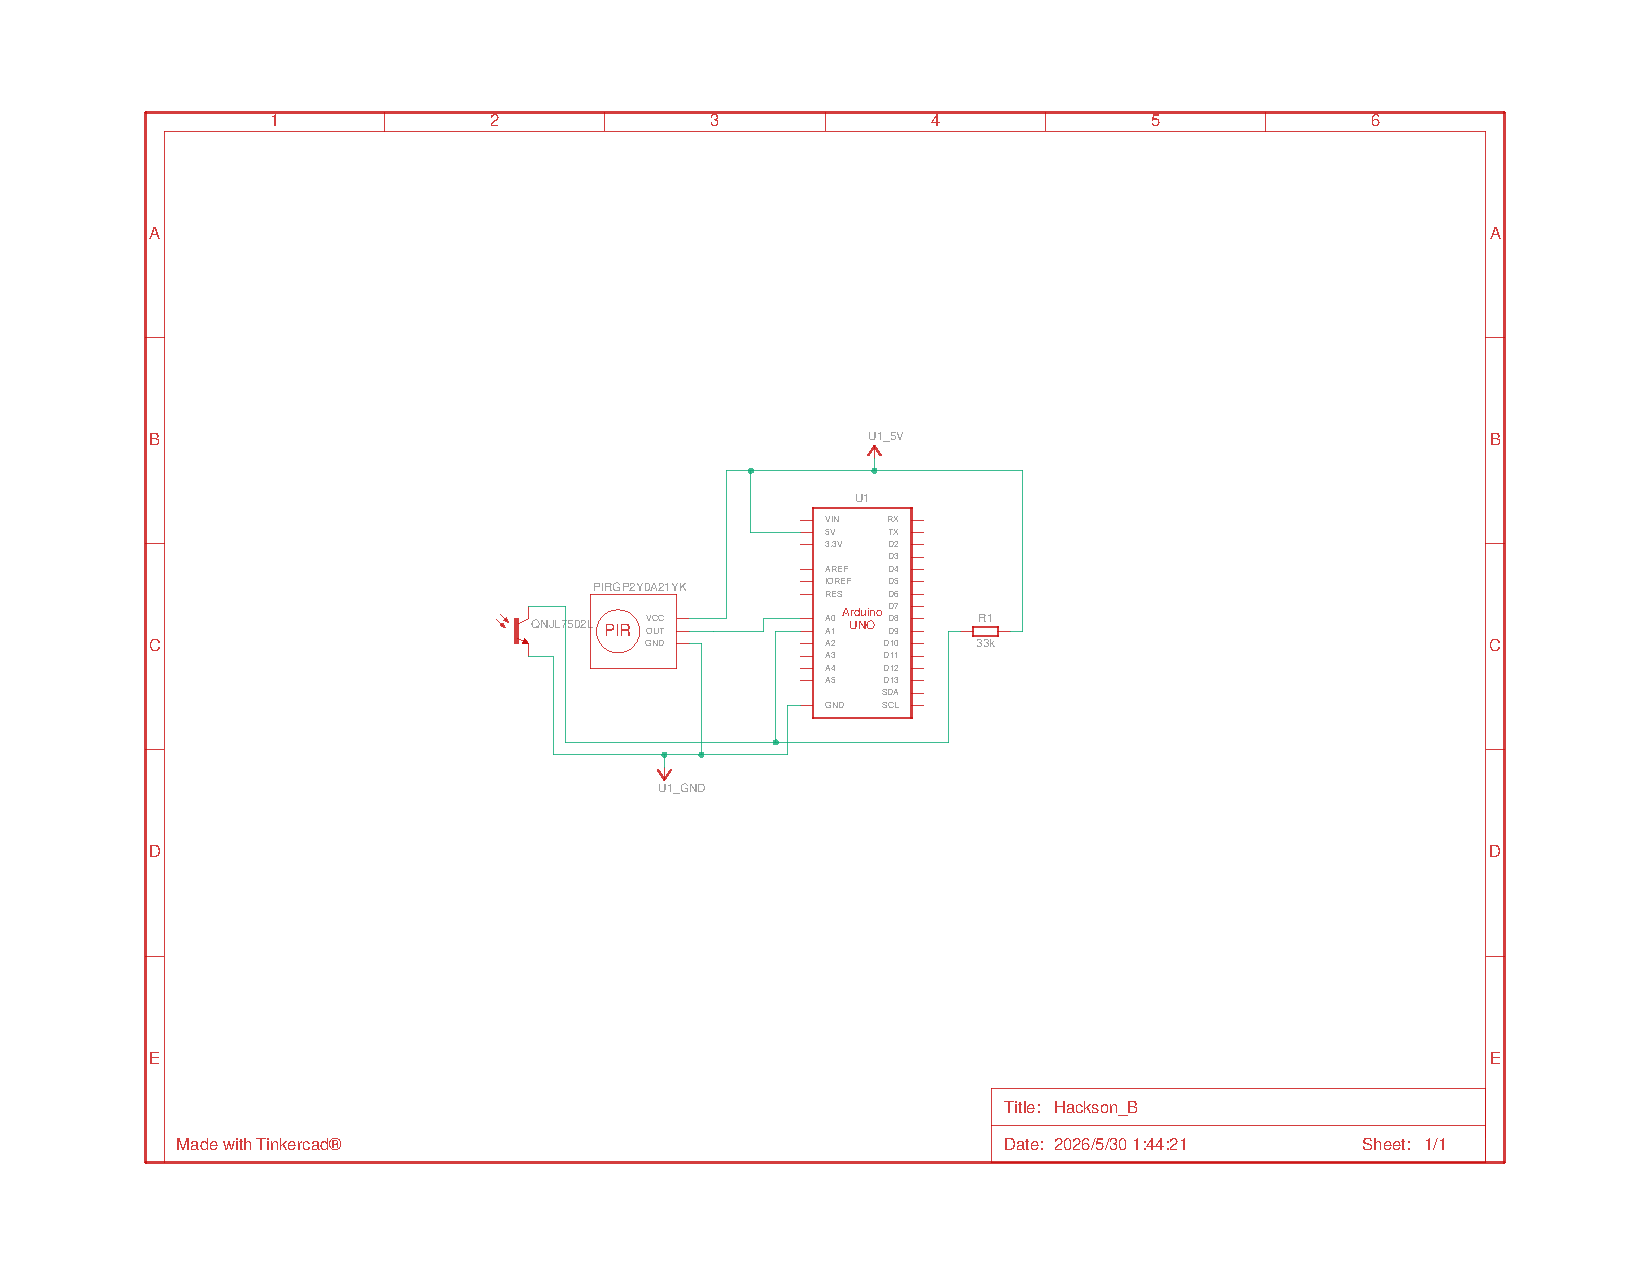
\includegraphics[width=0.8\linewidth]{figures/tantoB/Kairo_B.pdf}
\caption{回路図}
\label{fig:circuit_B}
\end{figure}

\subsection{ソフトウェア設計}

\subsubsection{ファイル構成}

\begin{table}[H]
\centering
\caption{ファイル構成}
\begin{tabular}{p{5cm}p{8cm}}
\hline
\textbf{ファイル名} & \textbf{内容} \\
\hline
\texttt{hackson\_main.ino} & BとCの共通部分．\texttt{setup()} および \texttt{loop()} のエントリポイント，共有変数の宣言，カラーセンサの初期化を含む． \\
\hline
\texttt{B.ino} & 担当Bの独立部分．フォトトランジスタポーリング・カラーセンサ判別・テンポ推定・状態機械の実装． \\
\hline
\texttt{C.ino} & 担当Cの独立部分．発音タイミング制御・シリアル送信の実装． \\
\hline
\texttt{AE\_S13683\_LED.h / .cpp} & カラーセンサ（AE\_S13683\_LED）のドライバライブラリ． \\
\hline
\end{tabular}
\end{table}

\subsubsection{オブジェクト設計（主要変数）}

\begin{lstlisting}[caption=担当 B 主要変数（B.ino / hackson\_main.ino）]
// ---- hackson_main.ino で宣言（担当Cと共有） ----
unsigned long          nextBeatTime    = 0;    // 次の拍予測絶対時刻 [ms]
volatile unsigned long currentBeatTime = 0;    // 現在の拍検出時刻 [ms]
volatile unsigned long lastBeatTime    = 0;    // 最後の拍検出時刻 [ms]
bool                   beatUpdated     = false; // nextBeatTime 更新フラグ
bool                   isPlaying       = false; // 演奏開始フラグ
enum                   State           {IDLE, PREBEAT, PLAYING};
State                  state           = IDLE;  // 現在の状態

// ---- B.ino で宣言（担当B専用） ----
// カラーセンサ
const char* colorName       = "Unknown"; // 検出した色名
const char* PLAY_COLOR_NAME = "Red";     // 自楽器の演奏開始色（楽器ごとに変更する）

// フォトトランジスタ
volatile bool beatDetected = false; // 拍検出フラグ（1ループで1回処理後リセット）
int           detectCount  = 0;     // 累積拍検出回数
bool          high         = false; // 現在のデジタル読み取り値
bool          stateHigh    = false; // 立ち上がりエッジ検出用フラグ

// EMA テンポ推定
float         estimatedBeatInterval = 1000.0f; // 推定拍間隔 [ms]
float         emaAlpha              = 0.2f;     // EMA 係数
unsigned long previousBeatTime      = 0;        // 前回拍検出時刻 [ms]
const float   TEMPO_CHANGE_THRESH   = 10.0f;   // テンポ急変検出閾値 [%]
float         previousNextBeatTime  = 0;        // 前回予測次拍時刻

// 状態機械
int       prebeatCount       = 0; // 予備振り中の拍検出回数
const int PREBEAT_THRESH     = 4; // 予備振り必要回数
const int MISSED_BEAT_THRESH = 3; // 演奏停止判定の未検出拍数倍率
\end{lstlisting}

\subsubsection{担当Cとの共有変数}

担当 B と担当 C は同一の Arduino 上で動作するため，以下のグローバル変数を共有することで連携する．
担当 B が書き込み，担当 C が読み取る変数を以下に示す．

\begin{table}[H]
\centering
\caption{担当 C との共有変数一覧}
\begin{tabular}{p{3.5cm}p{2.5cm}p{4cm}p{4cm}}
\hline
\textbf{変数名} & \textbf{型} & \textbf{担当Bの役割} & \textbf{担当Cの使い方} \\
\hline
\texttt{nextBeatTime} & \texttt{unsigned long} &
次の拍の予測絶対時刻を書き込む & 信号送信タイミングの基準として読む \\
\hline
\texttt{beatUpdated} & \texttt{bool} &
\texttt{nextBeatTime} が更新されたら \texttt{true} にする &
\texttt{true} を検知して処理後 \texttt{false} に戻す \\
\hline
\texttt{state} & \texttt{State} &
現在の演奏状態を書き込む &
IDLE 判定などに使う \\
\hline
\texttt{isPlaying} & \texttt{bool} &
カラーキュー一致時に \texttt{true} にする &
演奏開始のトリガーとして使う \\
\hline
\texttt{currentBeatTime} & \texttt{unsigned long} &
現在の拍検出時刻を書き込む &
\texttt{sendTime} 補正計算に使う \\
\hline
\end{tabular}
\end{table}

なお，\texttt{beatUpdated} を \texttt{false} にリセットする責任は担当 C 側にある．

\subsubsection{関数設計}

\begin{table}[H]
\centering
\footnotesize
\setlength{\tabcolsep}{3pt}
\renewcommand{\arraystretch}{1.1}
\caption{担当 B 主要関数一覧}
\label{tab:func_B}
\resizebox{\textwidth}{!}{%
\begin{tabular}{p{3.8cm}p{3.2cm}p{3.2cm}p{5.2cm}}
\hline
\textbf{関数名} & \textbf{入力} & \textbf{出力} & \textbf{役割} \\
\hline
\texttt{void photoISR()} &
PHOTO\_PIN（D4） &
high, stateHigh,
beatDetected,
currentBeatTime,
lastBeatTime &
デジタルピンをポーリングし，LOW→HIGHの立ち上がりエッジで拍を検出する．
前回検出から200\,ms以内は無視する（チャタリング防止）． \\
\hline
\texttt{const char*} \texttt{detectColor} \texttt{(float r,} \texttt{float g,} \texttt{float b)} &
RGB浮動小数点値 &
色名文字列（戻り値） &
入力RGB値を正規化し，7種の参照色（Red / Green / Blue / Yellow / Cyan / Magenta / White）とのコサイン類似度を計算して最も類似した色名を返す． \\
\hline
\texttt{void readColor()} &
カラーセンサ（I2C） &
colorName &
カラーセンサからワンショット測定でRGBを取得し，detectColor()で色名に変換してcolorNameを更新する．拍検出時のみ呼び出す． \\
\hline
\texttt{void updateTempoByPhoto()} &
currentBeatTime,
previousBeatTime,
estimatedBeatInterval,
state &
estimatedBeatInterval,
previousBeatTime,
nextBeatTime,
previousNextBeatTime &
拍間隔をEMAでテンポ推定する．
PLAYING状態かつ誤差率がTEMPO\_CHANGE\_THRESH（10\%）を超えた場合はEMAをバイパスして実測値を直接採用する．PREBEAT状態では常にEMAを適用する． \\
\hline
\texttt{void updateState()} &
beatDetected,
detectCount,
prebeatCount,
lastBeatTime,
estimatedBeatInterval &
state,
isPlaying,
prebeatCount &
IDLE / PREBEAT / PLAYINGの3状態を管理する．
各状態の遷移条件を判定し，stateを更新する． \\
\hline
\texttt{void B\_loop()} &
— &
— &
担当Bのメインループ処理．
photoISR()呼び出し→拍検出時のカラー判別・テンポ更新→状態遷移の順に実行する． \\
\hline
\end{tabular}
}
\end{table}

\subsection{処理フローの設計}

\begin{figure}[H]
  \centering
  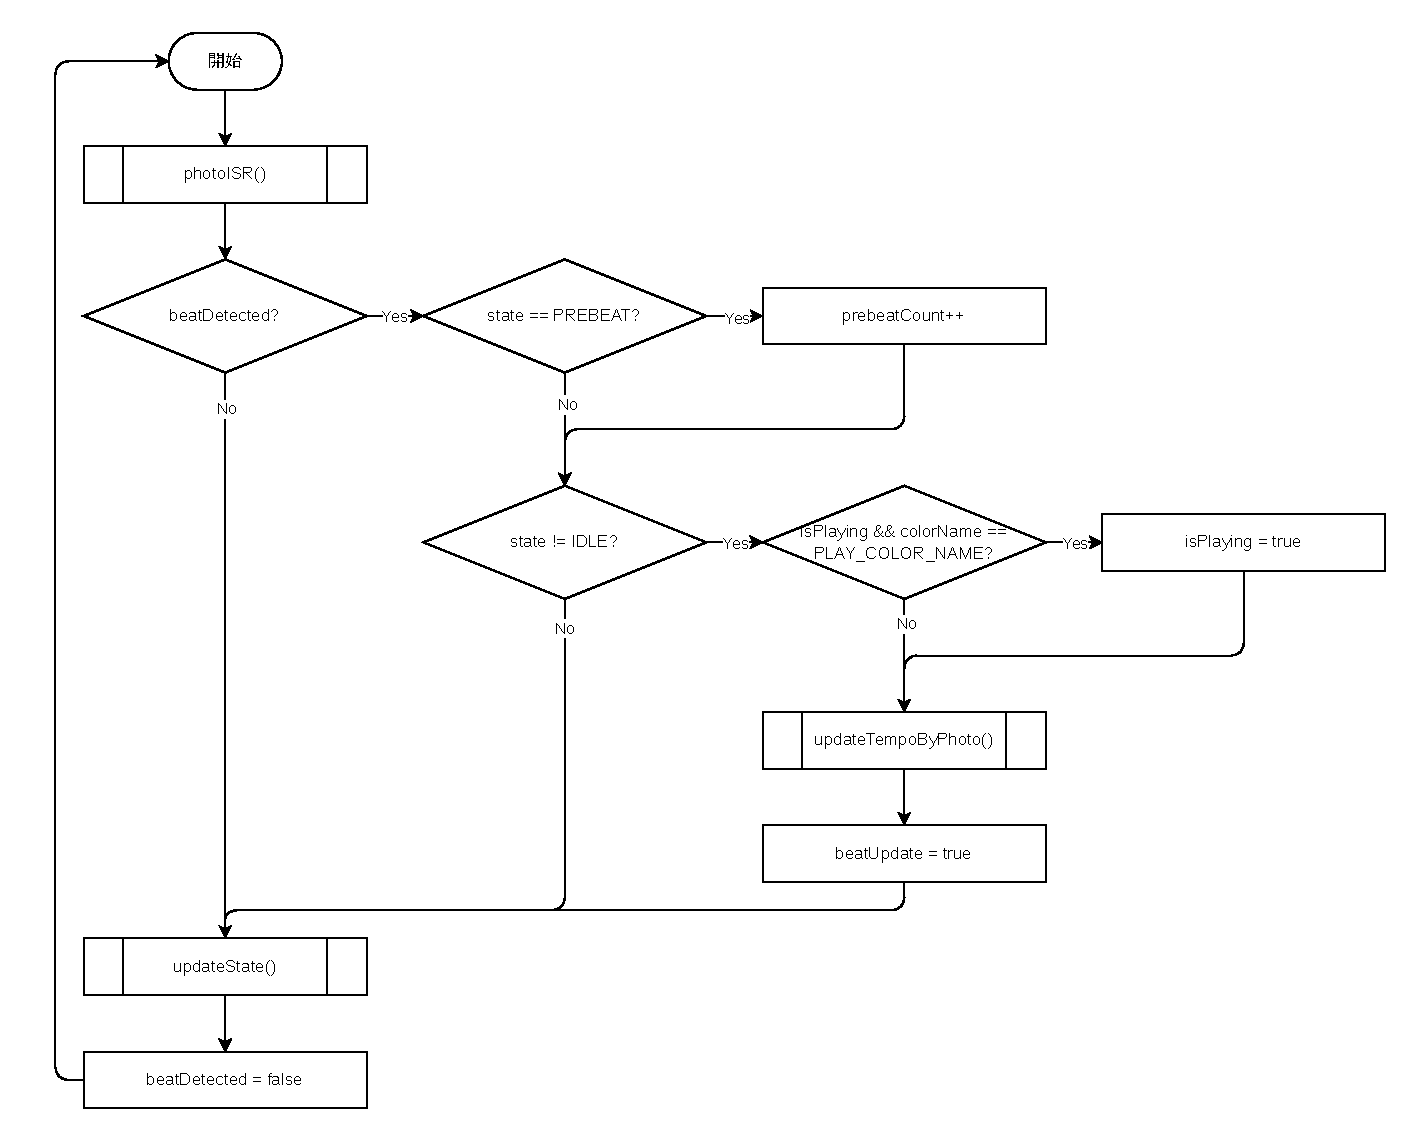
\includegraphics[width=0.8\linewidth]{figures/tantoB/flowchart_B_loop.pdf}
  \caption{B\_loop}
\end{figure}

\begin{figure}[H]
  \centering
  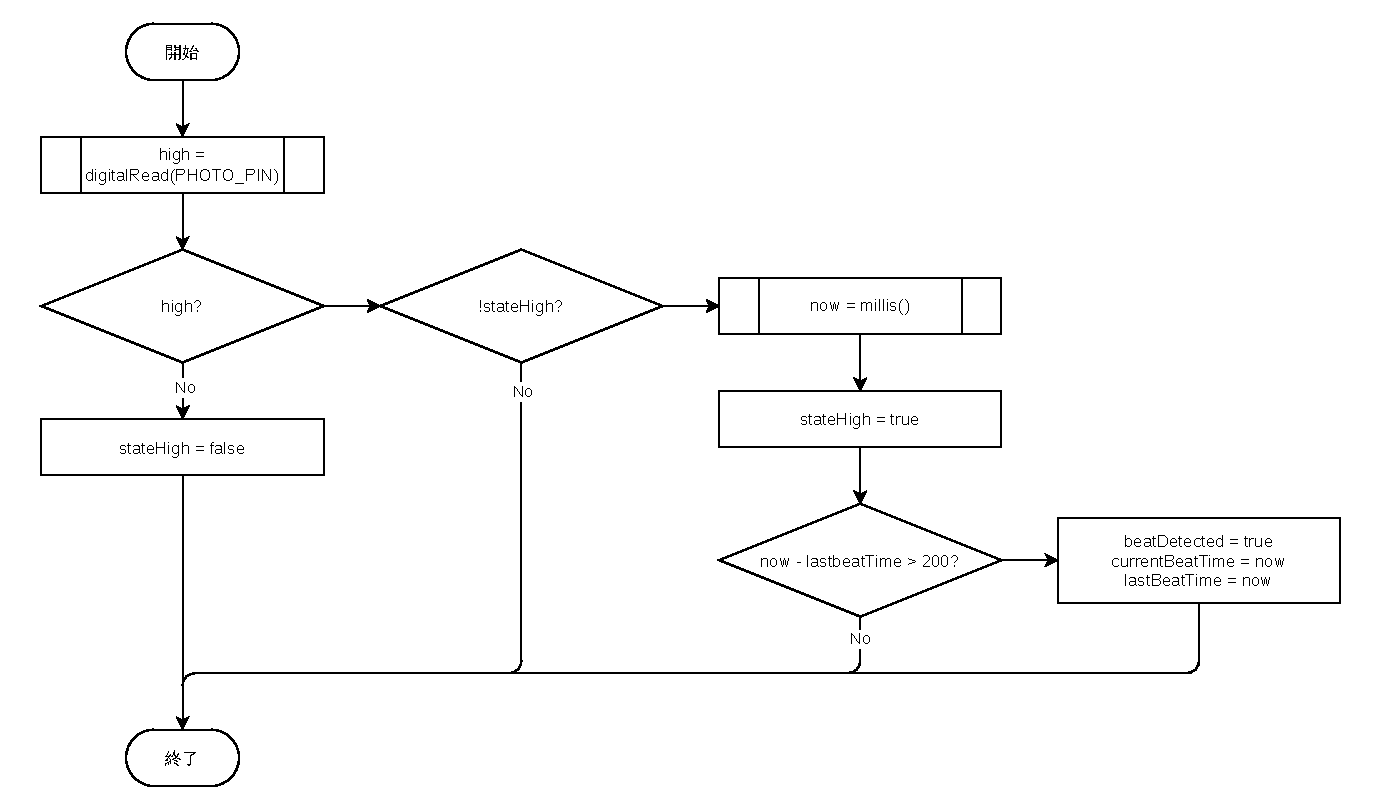
\includegraphics[width=0.8\linewidth]{figures/tantoB/flowchart_photoISR.pdf}
  \caption{photoISR}
\end{figure}

\begin{figure}[H]
  \centering
  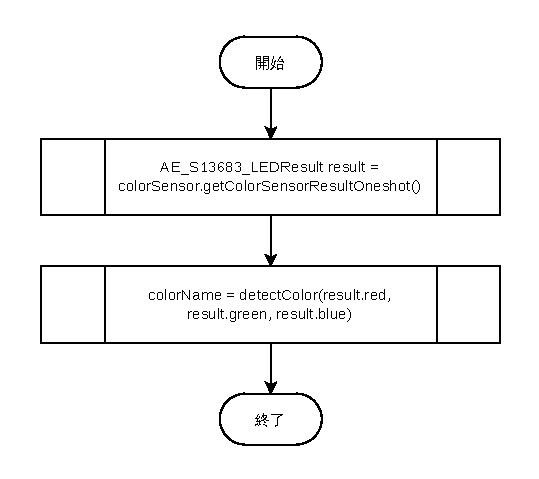
\includegraphics[width=0.8\linewidth]{figures/tantoB/flowchart_readColor.pdf}
  \caption{readColor}
\end{figure}

\begin{figure}[H]
  \centering
  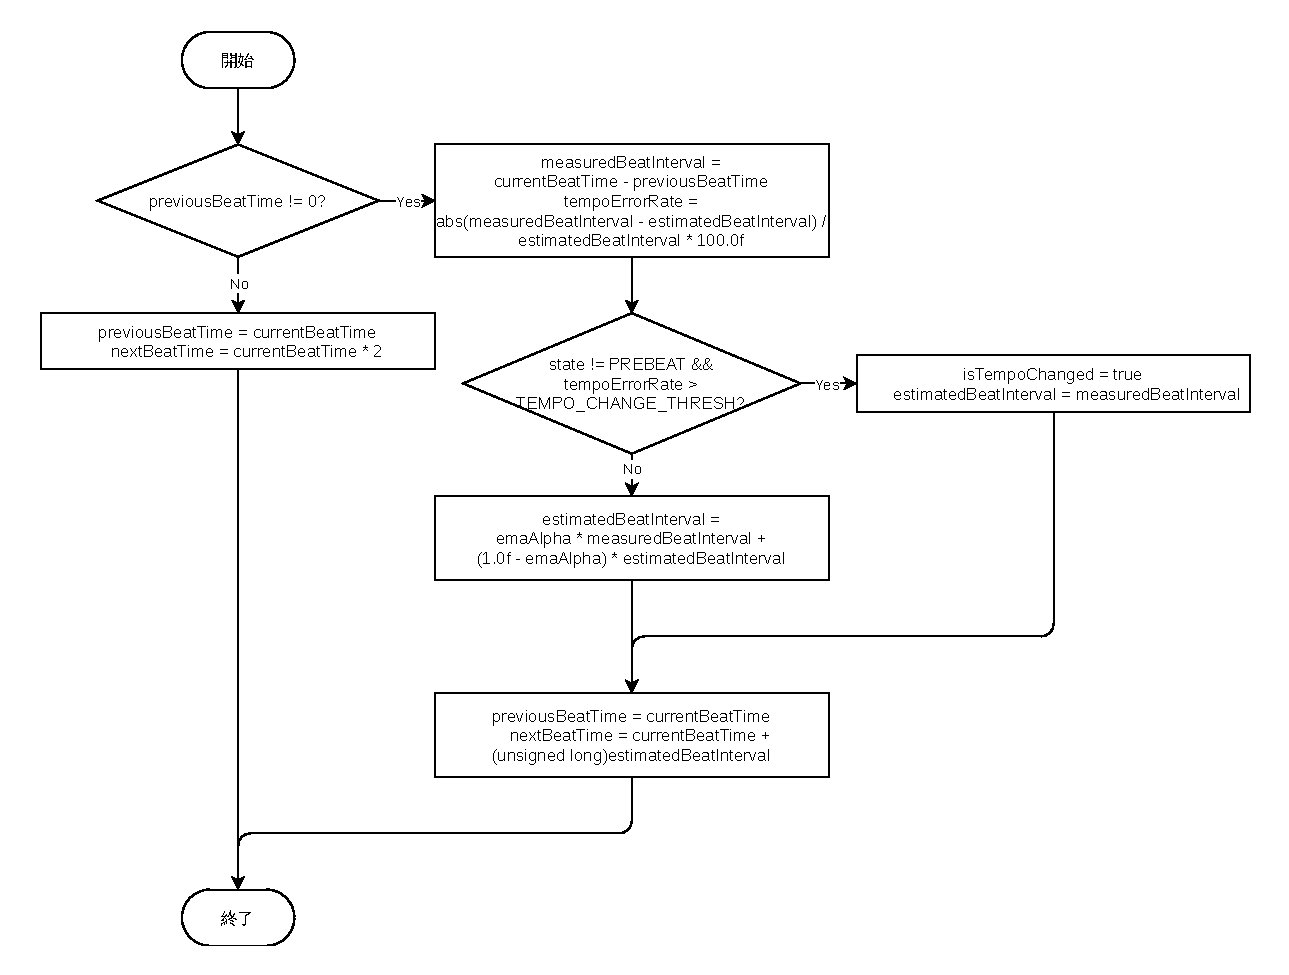
\includegraphics[width=0.8\linewidth]{figures/tantoB/flowchart_updateTempoByPhoto.pdf}
  \caption{updateTempoByPhoto}
\end{figure}

\begin{figure}[H]
  \centering
  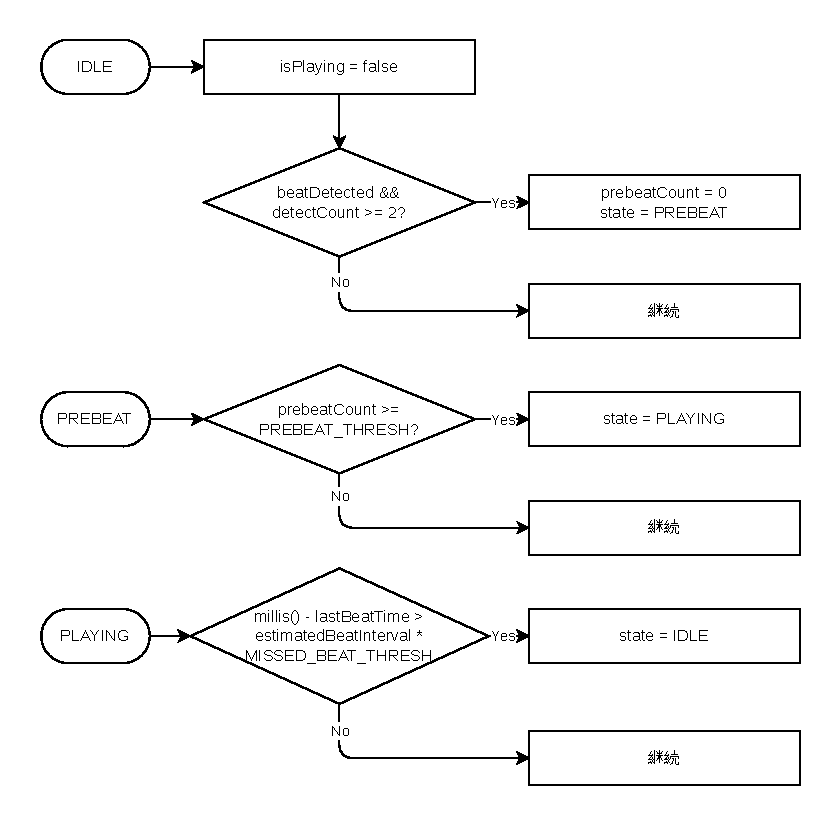
\includegraphics[width=0.8\linewidth]{figures/tantoB/flowchart_updateState.pdf}
  \caption{updateState}
\end{figure}

\subsection{テストの設計}

担当Bが実施すべきテストの一覧を表\ref{tab:test_B}に示す．

\begin{table}[H]
\centering
\caption{テスト一覧}
\label{tab:test_B}
\begin{tabular}{p{3.5cm}p{5cm}p{4cm}}
\hline
\textbf{テスト名} & \textbf{内容} & \textbf{合格基準} \\
\hline
拍検出精度確認 &
指揮者LEDをメトロノームに合わせて点滅させ，
\texttt{photoISR()}が正しく拍を検出するか確認する．
また200\,ms以内の再検知が無視されることを確認する． &
検出成功率95\%以上，誤検出なし \\
\hline
カラーキュー判別確認 &
各楽器に対応する色（Red/Green/Blue/Yellow/White）を親機LEDで発光させ，
\texttt{detectColor()}が正しい色名を返すか確認する．
またシリアルモニタで \texttt{colorName} を観察する． &
5色全て正しく判別，誤判別なし \\
\hline
EMAテンポ推定精度確認 &
メトロノーム（80\,bpm，104\,bpm）に合わせて指揮動作を行い，
シリアルモニタで \texttt{estimatedBeatInterval} から換算したBPMを計測する． &
BPM誤差 $\pm$5\,bpm以内 \\
\hline
状態機械遷移確認 &
3状態の遷移シーケンスをシリアルモニタでトレースする．
IDLE→PREBEAT→PLAYINGおよびPLAYING→IDLEを確認する． &
設計通りの遷移のみ発生，無効遷移なし \\
\hline
演奏開始フラグ連携確認 &
\texttt{isPlaying}フラグが立った直後に担当Cが演奏パケットを送信するか確認する． &
色検出から1拍以内に演奏開始 \\
\hline
B-C間遅延測定（結合） &
拍検出タイムスタンプとNOTE\_ON送信タイムスタンプの差をシリアルで計測する． &
遅延 $\leq$50\,ms \\
\hline
A-B間テンポ追従確認（結合） &
人形BPMを80→104に変化させ，担当BのEMAが追従するか確認する． &
3小節以内に新テンポに収束 \\
\hline
\end{tabular}
\end{table}
